 %GPL V3 by Mathias Hablützel, feel free to improve this template
 \documentclass[a4paper,10pt]{article}
 
 % Use UTF8 since the laptop is configured so and use ngerman for word breaking.
 % If you encounter an encoding problem, remove the line with utf8.
 \usepackage[utf8]{inputenc}
 \usepackage[ngerman]{babel}
 \usepackage[pdftex]{graphicx}
 
 % TikZ für schöne Grafiken und so.
 \usepackage{tikz}
 \usetikzlibrary{positioning,calc,fadings,decorations.pathreplacing,arrows}
 \usepackage{pgfplots}

% \usepackage{hyperref}
 \usepackage{colortbl}
 \usepackage{tabularx}
 \usepackage{color}
 \usepackage{amsfonts}
 \usepackage{amsmath}
 \usepackage{gensymb}
 \usepackage{listings}
 \usepackage{multirow}
 \usepackage{fancyhdr}
 \usepackage{multicol}
 \usepackage{wrapfig}
 \usepackage{pdfpages}
 \usepackage[colorlinks=true,
  linkcolor=black,
  citecolor=black,
  filecolor=black,
  pagecolor=black,
  urlcolor=black,
  bookmarks=true,
  bookmarksopen=true,
  bookmarksopenlevel=3,
  plainpages=false,
  pdfpagelabels=true]{hyperref}

% Hack for german umlaute
\lstset{
  literate={ö}{{\"o}}1
           {ä}{{\"a}}1
           {ü}{{\"u}}1
}

% define colors
 \definecolor{hellgrau}{rgb}{0.8,0.8,0.8}

  % http://stackoverflow.com/questions/741985/latex-source-code-listing-like-in-professional-books
  \usepackage{listings}
  \usepackage{courier}
 \lstset{
         basicstyle=\footnotesize\ttfamily, % Standardschrift
         numbers=left,               % Ort der Zeilennummern
         numberstyle=\tiny,          % Stil der Zeilennummern
         stepnumber=1,               % Abstand zwischen den Zeilennummern
         numbersep=5pt,              % Abstand der Nummern zum Text
         tabsize=2,                  % Groesse von Tabs
         extendedchars=true,         %
         breaklines=true,            % Zeilen werden Umgebrochen
         keywordstyle=\color{red},
    		frame=b,         
 %        keywordstyle=[1]\textbf,    % Stil der Keywords
 %        keywordstyle=[2]\textbf,    %
 %        keywordstyle=[3]\textbf,    %
 %        keywordstyle=[4]\textbf,   \sqrt{\sqrt{}} %
         stringstyle=\color{white}\ttfamily, % Farbe der String
         showspaces=false,           % Leerzeichen anzeigen ?
         showtabs=false,             % Tabs anzeigen ?
         xleftmargin=17pt,
         framexleftmargin=17pt,
         framexrightmargin=5pt,
         framexbottommargin=4pt,
         %backgroundcolor=\color{lightgray},
         showstringspaces=false      % Leerzeichen in Strings anzeigen ?        
 }
 \lstloadlanguages{% Check Dokumentation for further languages ...
         %[Visual]Basic
         %Pascal
         %C
         %C++
         %XML
         %HTML
         Java
 }
    %\DeclareCaptionFont{blue}{\color{blue}} 

  %\captionsetup[lstlisting]{singlelinecheck=false, labelfont={blue}, textfont={blue}}
  \usepackage{caption}
\DeclareCaptionFont{white}{\color{white}}
\DeclareCaptionFormat{listing}{\colorbox[cmyk]{0.43, 0.35, 0.35,0.01}{\parbox{\textwidth}{\hspace{15pt}#1#2#3}}}
\captionsetup[lstlisting]{format=listing,labelfont=white,textfont=white, singlelinecheck=false, margin=0pt, font={bf,footnotesize}}


 % I set here a different sidemargin because the original margin looks not so
 % good for normal documents. Additionally I have to enlarge the textwidth.
 \setlength{\oddsidemargin}{0cm}
 \setlength{\evensidemargin}{0cm}
 \addtolength{\textwidth}{4cm}
\newcolumntype{C}[1]{>{\centering\arraybackslash}m{#1}} 

\begin{document} 
 % Here I use the up-to-date font encoding T1 and the font familly Computer Modern
 % Sans Serif (since I don't like the standard font) medium and normal (non-italic or so).
 \usefont{T1}{cmss}{m}{n}

\pagestyle{fancy} %eigener Seitenstil
\fancyhf{} %alle Kopf- und Fußzeilenfelder bereinigen
\fancyhead[C]{LakeRouting - Optimale Wegfindung anhand von Wettermodellen} %zentrierte Kopfzeile
\renewcommand{\headrulewidth}{0.4pt} 
\fancyfoot[C]{\thepage}

 \title{\begin{flushleft}\vspace*{-3cm}
\includegraphics[keepaspectratio,width=7cm]{img/de-zhaw-cmyk}\end{flushleft} \vspace*{4cm} LakeRouting - Optimale Wegfindung anhand von Wettermodellen }
 \date{\today}
 \author{Fevzi Yükseldi (yuksefev@students.zhaw.ch)\\
 Mathias Hablützel (hablumat@students.zhaw.ch)\\
 \\
Dr. Rudolf M. Füchslin (furu@zhaw.ch)\\
Jacques Ambühl (jacques.ambuehl@meteoschweiz.ch)}
 
 \maketitle
\thispagestyle{empty}
 \newpage
\thispagestyle{empty}
\part*{Management Summary}

\vspace*{2cm}
\setlength{\columnsep}{2cm}
\begin{multicols}{2}

\textbf{\textsc{Deutsch}}
\vspace{1cm}\\

\columnbreak

\textbf{\textsc{English}}
\vspace{1cm}\\

\end{multicols}
\newpage

\cleardoublepage
\begingroup
\pagestyle{empty}
\setcounter{tocdepth}{2}
\tableofcontents
\clearpage
\endgroup
       
\newpage

\setcounter{page}{1} 
\part{Einleitung}
\section{Ausgangslage}
Zu den klassischen Methoden der mathematischen Entscheidungsvorbereitung gehört die Dynamische Programmierung (DP). Sie ermöglicht die optimale Gestaltung einer Kette sequentieller Entscheidungen aufgrund wettbewerbsrelevanter Randbedingungen (physikalischer oder ökonomischer Natur).\\
...
% Geschichtliche Entwicklung
% Stand der Technik
% Kurz den Industriepartner nennen.


\section{Ziel / Auftrag}
Die vorgeschlagene Bachelorarbeit schlägt eine Anwendung der DP zur
Kursbestimmung eines Segelschiffs vor. Aufgrund der mit einem
numerischen Modell vorausgesagten Wetterentwicklung und in Anbetracht
der Leistungskurve (Polardiagramm) des Schiffes wird dessen optimale
Route mittels DP gerechnet. Ähnliche Methoden wurden beim Alinghi Team
im Rahmen des Americas Cup verwendet.

Weitere Anwendungen der DP zum Thema ''energy trading'' für erneuerbare
Energiequellen sind denkbar und eine Übertragung der Resultate der BA in
diesen Bereich werden von MeteoSchweiz angestrebt.

% Anforderungen an das Resultat der Arbeit

\subsection{Terminologie}
% Definiert die in der Arbeit verwendeten Begriffe
\paragraph{Seemeile}ist eine in der Meteorologie gebräuchliche Längeneinheit, die als Berechnungsgrundlage für die Navigation und das Angeben von Distanzen dient. Sie entspricht der Länge einer Winkelminute auf einer Sphäre und auf der Erde beträgt diese Distanz 1852 m.
\paragraph{Winkelminute}ist der sechzigste Teil eines Winkelgrades, welches wiederum der dreihundertsechzigste Teil einer Umdrehung ist. Somit wäre eine Winkelminute \\ \( W=\frac{1 Grad}{60} = 0.0\overline{16}^\circ \)
\paragraph{Knoten}ist ein Geschwindigkeitsmass in der Meteorologie, das auf der Längeneinheit Seemeile beruht. Somit ist ein Knoten 1852 m/h = 0.514 m/s.


\section{Weitere Informationen sowie Danksagung}
Für die professionelle und freundliche Kooperation möchten wir uns an
dieser Stelle herzlich bedanken!\\
...

\newpage
\part{Vorgehen / Methoden}
\section{Dynamische Programmierung}
Der Begriff dynamische Programmierung wurde erstmals in den 1940er Jahren von
Richard Bellman benutzt und umfasst eine Reihe von Methoden mit dem Ziel,
Optimierungsprobleme zu lösen. 

Das Optimierungsproblem wird dann erfolgreich mit diesem Verfahren gelöst, wenn
sie in mehrere gleichartige Teilprobleme aufgeteilt werden kann. Eine optimale
Lösung setzt sich somit aus den optimalen Lösungen der Teilproblemen zusammen.
Aus diesem Grund ist eine Strategie dann optimal, wenn alle Unterstrategien
optimal sind. Die Zwischenergebnisse der Teilprobleme werden aber nicht
rekursiv, sondern iterativ berechnet und in einer Tabelle gespeichert, so dass,
wenn sie wieder benötigt werden, nicht nochmals berechnet werden müssen.

In unserer Anwendung ist das Ziel klar: Den Kurs des Segelschiffes bestimmen
indem man die kürzeste Route vom Start- bis zum Endpunkt berechnet. Dies
erfolgt indem man die Strecke in Teilstrecken aufteilt und die Dauer der Fahrt
für diese Strecken berechnet. Danach wird der Pfad mit der kleinsten Dauer
bestimmt. Zu diesem Zweck werden die Windvektoren auf der Wasseroberfläche und
ihre Interaktion mit dem Segelschiff in die Berechnung miteinbezogen. 

\subsection{Die ersten Schritte}
Betrachten wir nun ein Fahrzeug, welches sich auf der Erdoberfläche mit einer
konstanten Geschwindigkteit bewegt. Nehmen wir an, dass dieses Fahrzeug von
einem Anfangspunkt bis zu einem Ankunftspunkt reisen möchte. Die Sequenzierung,
also die Zerstückelung der Strecke wird mit der Aufspannung eines Gitternetzes
zwischen diesen beiden Punkten bereitgestellt.

Beginnend mit einer sehr einfachen Formulierung, die schrittweise verfeinert
werden soll, definiert man:

\( \Delta t_i\;,  i=0...m\), ist die benötigte Zeit von der \( (i-1)\)-ten
Schicht bis zur \(i\)-ten Shicht, wobei \(i=0\) der ersten Schicht entspricht,
wo sich der Anfangspunkt befindet und \(i=m\) der letzten Schicht entspricht,
wo sich der Ankunftspunkt befindet.

\( D_i\;,  i=0...m\), bis zu der \(i\)-ten Schicht benötigte Zeit.

Unser optimales Programm kann somit wie folgt definiert werden: "Minimierung
der Reisedauer \(D_m\) von der Schicht \(0\) bis \(m\)". 

\begin{equation}
\label{eq_dyn:1}
D_m = \overset{m}{\underset{i=1}{\min}} [\; \sum_{i=1}^m \Delta t_i\;]
 \end{equation}
Wenn wir eine Zwischenstufe \(I\) berechnen lassen, erhalten wir die folgende, umgeschriebene Formel:
\begin{equation}
\label{eq_dyn:2}
D_I = \overset{I}{\underset{i=1}{\min}} [\; \Delta t_I + \sum_{i=1}^{I-1}
\Delta t_i\;] = \overset{I}{\min} [\; \Delta t_I +
\overset{I-1}{\underset{i=1}{\min}} [\; \sum_{i=1}^{I-1} \Delta t_i\;]\;] =
\overset{I}{\min} [\; \Delta t_I + D_{I-1} \;]
 \end{equation}
Somit liefert die Gleichsetzung der ersten und letzten Ausdrücke eine rekursive
Formulierung des Problems. Desweiteren muss ein Anfangswert angegeben werden,
vorausgesetzt \(D_0  = D_{i=0} =\) Abfahrtszeit ist, so dass gilt:
 
 \begin{equation}
\label{eq_dyn:3}
D_I =  \overset{I}{\min} [\; \Delta t_I + D_{I-1} \;];\;\;\;\;\;\; D_0: Abfahrtszeit.
 \end{equation}
 
Diese Ableitung ergibt sich aus einer tiefgründigen Optimierungsprinzip, dass
eine Strategie nur dann optimal ist, wenn alle ihre Unterstrategien optimal
sind. Und somit birgt eine solche pauschale Formulierung den
Entscheidungsprozess. 
 
Folglich gibt es zwei Entscheidungsverfahren:\\ \\
- Bei jedem Knoten j in der Schicht I-1 soll eine Abfrage durchgeführt werden, zu welchem Knoten k in der nächsten Schicht I das Segelschiff segeln soll.\\
oder\\
- Bei jedem Knoten k in der Schicht I soll eine Abfrage durchgeführt werden, von welchem Knoten j in der vorherigen Schicht I-1 das Segelschiff gesegelt haben soll.\\

Die Einführung in die letzte Bedingung im vorherigen Ausdruck für \(D_I\)  ergibt (mit Standard-Typografie \{i,j\}  für die Darstellung von Knoten in der Graphentheorie):
\begin{equation}
\label{eq_dyn:4}
D_{(I,k)} = \overset{j=n}{\underset{j=-n}{\min}} [\; \Delta t_{\{I-1,j\}}^{\{I,k\}} + D_{(I-1.j)} \;];\;\;\;\;\;\; D_0: Abfahrtszeit.
 \end{equation}%Eng
 The node j * belonging to the slice I-1 and satisfying the above minimum is the decision taken in the slice I for the node k. It is expressed as:%Eng
 \begin{equation}
\label{eq_dyn:5}
D_{(I,k)} \to j^* \in Schicht\; I-1
 \end{equation}
 
Es ist ersichtlich, dass der Ausdruck \(D\) - für die Dauer - auch sehr leicht für Decision (dt. Entscheidung) gehandelt werden kann. Mit dieser Annahme, beinhaltet der Ausdruck \(D_I\) in der Formel \eqref{eq_dyn:3} alle gewählten Entscheidungen der Schicht I, und dies für jeden Knoten k einzeln in dieser Schicht.

  \begin{equation}
\label{eq_dyn:6}
D_I \to \{\;j_{-n}^*\; ... \;j_{k}^* \;...\; j_{n}^*\;\} \subset Schicht\; I-1
 \end{equation}
Die Anzahl der Schritte vom Anfangspunkt bis zum Ankunftspunkt ist als \(m\) und die Anzahl der Zeilen (Optionen) als n definiert, welche auch später näher erläutert werden.
 
Eine weitere Verfeinerung muss eingeführt werden. Nehmen wir an, wir hätten ein Knoten mit dem Index \{i,-n\} ausgewählt. Somit ist es laut unserem Algorithmus möglich, dass der Vorgänger dieser Knotens den Index \{i-1,+n\} haben kann, was einer seitlichen Kreuzung entspricht und eher Unwahrscheinlich ist. \\
Deshalb braucht es ein Steuermechanismus, der die Anzahl der möglichen Adressierungen von einem Knoten \{i, k\} mit den Knoten der vorherigen Spalte \{i-1, k\} begrenzt. Dies wird mit dem Spread-Parameter erreicht und sieht dann wie folgt aus:

   \begin{equation}
\label{eq_dyn:7}
D_{I,k} \to j^*\; mit\; |\;j^*\;-\;k\;| \;\le\; Spread;\; j^*\; \in Schicht\; I-1
 \end{equation}
 
Somit werden nur die Knoten in der Schicht \(i\) als Nachbarn für die Knoten in der Schicht \(i-1\) gelten, welche auch diese Bedingung erfüllen. Die restlichen Knoten der Schicht \(i\), die diese Bedingung nicht erfüllen, werden einfach bei der Auswahl nicht berücksichtigt.

Der Spread-Parameter wird uns später auch einen weiteren Vorteil bringen, und zwar wird es uns helfen die Problematik mit der Küste zu bewältigen, so dass unsere Route nicht das Gewässer verlässt.

\newcommand\pgfmathsinandcos[3]{%
  \pgfmathsetmacro#1{sin(#3)}%
  \pgfmathsetmacro#2{cos(#3)}%
}

\newcommand\LongitudePlane[3][current plane]{%
  \pgfmathsinandcos\sinEl\cosEl{#2} % elevation
  \pgfmathsinandcos\sint\cost{#3} % azimuth
  \tikzset{#1/.estyle={cm={\cost,\sint*\sinEl,0,\cosEl,(0,0)}}}
}

\newcommand\LatitudePlane[3][current plane]{%
  \pgfmathsinandcos\sinEl\cosEl{#2} % elevation
  \pgfmathsinandcos\sint\cost{#3} % latitude
  \pgfmathsetmacro\yshift{\cosEl*\sint}
  \tikzset{#1/.estyle={cm={\cost,0,0,\cost*\sinEl,(0,\yshift)}}} %
}

\newcommand\DrawLongitudeCircle[2][1]{
  \LongitudePlane{\angEl}{#2}
  \tikzset{current plane/.prefix style={scale=#1}}
   % angle of "visibility"
  \pgfmathsetmacro\angVis{atan(sin(#2)*cos(\angEl)/sin(\angEl))} %
  \draw[current plane,thin,black] (\angVis:1) arc (\angVis:\angVis+180:1);
  \draw[current plane,thin,dashed] (\angVis-180:1) arc (\angVis-180:\angVis:1);
}%this is fake: for drawing the grid


\newcommand\DrawLongitudeCirclered[2][1]{
  \LongitudePlane{\angEl}{#2}
  \tikzset{current plane/.prefix style={scale=#1}}
   % angle of "visibility"
  \pgfmathsetmacro\angVis{atan(sin(#2)*cos(\angEl)/sin(\angEl))} %
  \draw[current plane,red,thick] (150:1) arc (150:180:1);
  %\draw[current plane,dashed] (-50:1) arc (-50:-35:1);
}%for drawing the grid


\newcommand\DLongredd[2][1]{
  \LongitudePlane{\angEl}{#2}
  \tikzset{current plane/.prefix style={scale=#1}}
   % angle of "visibility"
  \pgfmathsetmacro\angVis{atan(sin(#2)*cos(\angEl)/sin(\angEl))} %
  \draw[current plane,black,dashed, ultra thick] (150:1) arc (150:180:1);
}


\newcommand\DLatred[2][1]{
  \LatitudePlane{\angEl}{#2}
  \tikzset{current plane/.prefix style={scale=#1}}
  \pgfmathsetmacro\sinVis{sin(#2)/cos(#2)*sin(\angEl)/cos(\angEl)}
  % angle of "visibility"
  \pgfmathsetmacro\angVis{asin(min(1,max(\sinVis,-1)))}
  \draw[current plane,dashed,black,ultra thick] (-50:1) arc (-50:-35:1);
}


\newcommand\fillred[2][1]{
  \LongitudePlane{\angEl}{#2}
  \tikzset{current plane/.prefix style={scale=#1}}
   % angle of "visibility"
  \pgfmathsetmacro\angVis{atan(sin(#2)*cos(\angEl)/sin(\angEl))} %
  \draw[current plane,red,thin] (\angVis:1) arc (\angVis:\angVis+180:1);
}

\newcommand\DrawLatitudeCircle[2][1]{
  \LatitudePlane{\angEl}{#2}
  \tikzset{current plane/.prefix style={scale=#1}}
  \pgfmathsetmacro\sinVis{sin(#2)/cos(#2)*sin(\angEl)/cos(\angEl)}
  % angle of "visibility"
  \pgfmathsetmacro\angVis{asin(min(1,max(\sinVis,-1)))}
  \draw[current plane,thin,black] (\angVis:1) arc (\angVis:-\angVis-180:1);
  \draw[current plane,thin,dashed] (180-\angVis:1) arc (180-\angVis:\angVis:1);
}%Defining functions to draw limited latitude circles (for the red mesh)


\newcommand\DrawLatitudeCirclered[2][1]{
  \LatitudePlane{\angEl}{#2}
  \tikzset{current plane/.prefix style={scale=#1}}
  \pgfmathsetmacro\sinVis{sin(#2)/cos(#2)*sin(\angEl)/cos(\angEl)}
  % angle of "visibility"
  \pgfmathsetmacro\angVis{asin(min(1,max(\sinVis,-1)))}
  %\draw[current plane,red,thick] (-\angVis-50:1) arc (-\angVis-50:-\angVis-20:1);
\draw[current plane,red,thick] (-50:1) arc (-50:-35:1);
}


\tikzset{
  >=latex,
  inner sep=0pt,
  outer sep=2pt,
  mark coordinate/.style={inner sep=0pt,outer sep=0pt,minimum size=3pt, fill=black,circle}
}


\section{Aufgabe 1 - Orthodromie}
\subsection{Aufgabenstellung}
\begin{itemize}
  \item Erstellung eines Entscheidungsnetzes auf der Erdkugel
  \item Berechnung einer Orthodromie (Distanz in Meilen zwischen zwei Punkten auf der Erdkugel)
  \item Erstellung der Koordinatendatei eines Sees (in Koordinaten)
\end{itemize}

\subsection{Analyse der Problemstellung}
Auf einer Kugel soll zwischen zwei Punkten die kürzeste Route bzw. die kürzeste Verbindung gewählt werden. Dies wird durch das Vektorprodukt der beiden Vektoren vom Kugelursprung zu den beiden Punkten $A$ und $B$ einfach berechnet:

\begin{tikzpicture}[scale=1,every node/.style={minimum size=1cm}]
	%% some definitions
	
	\def\R{4} % sphere radius
	
	\def\angEl{25} % elevation angle
	\def\angAz{-100} % azimuth angle
	\def\angPhiOne{-50} % longitude of point P
	\def\angPhiTwo{-15} % longitude of point Q
	\def\angBeta{30} % latitude of point P and Q
	
	%% working planes
	
	\pgfmathsetmacro\H{\R*cos(\angEl)} % distance to north pole
	\LongitudePlane[xzplane]{\angEl}{\angAz}
	\LongitudePlane[pzplane]{\angEl}{\angPhiOne}
	\LongitudePlane[qzplane]{\angEl}{\angPhiTwo}
	\LatitudePlane[equator]{\angEl}{0}
	\fill[ball color=white!10] (0,0) circle (\R); % 3D lighting effect
	\coordinate (O) at (0,0);
	\coordinate[mark coordinate] (N) at (0,\H);
	\coordinate[mark coordinate] (S) at (0,-\H);
	
    \DrawLongitudeCircle[\R]{\angPhiOne} % pzplane
    \DrawLongitudeCircle[\R]{\angPhiTwo} % qzplane
    \DrawLatitudeCircle[\R]{\angBeta}
    \DrawLatitudeCircle[\R]{0} % equator
	%labelling north and south
	\node[above=8pt] at (N) {$\mathbf{N}$};
	\node[below=8pt] at (S) {$\mathbf{S}$};
        \draw[-,dashed, thick] (N) -- (S);	
    	
\end{tikzpicture}


% Author: Mathias Hablützel

\section{Erfassung Schiffsgeschwindigkeiten}

\subsection{Problemanalyse}
\subsubsection{Windangriffswinkel und Windgeschwindigkeit}

\begin{wrapfigure}{r}{6cm} 
\centering
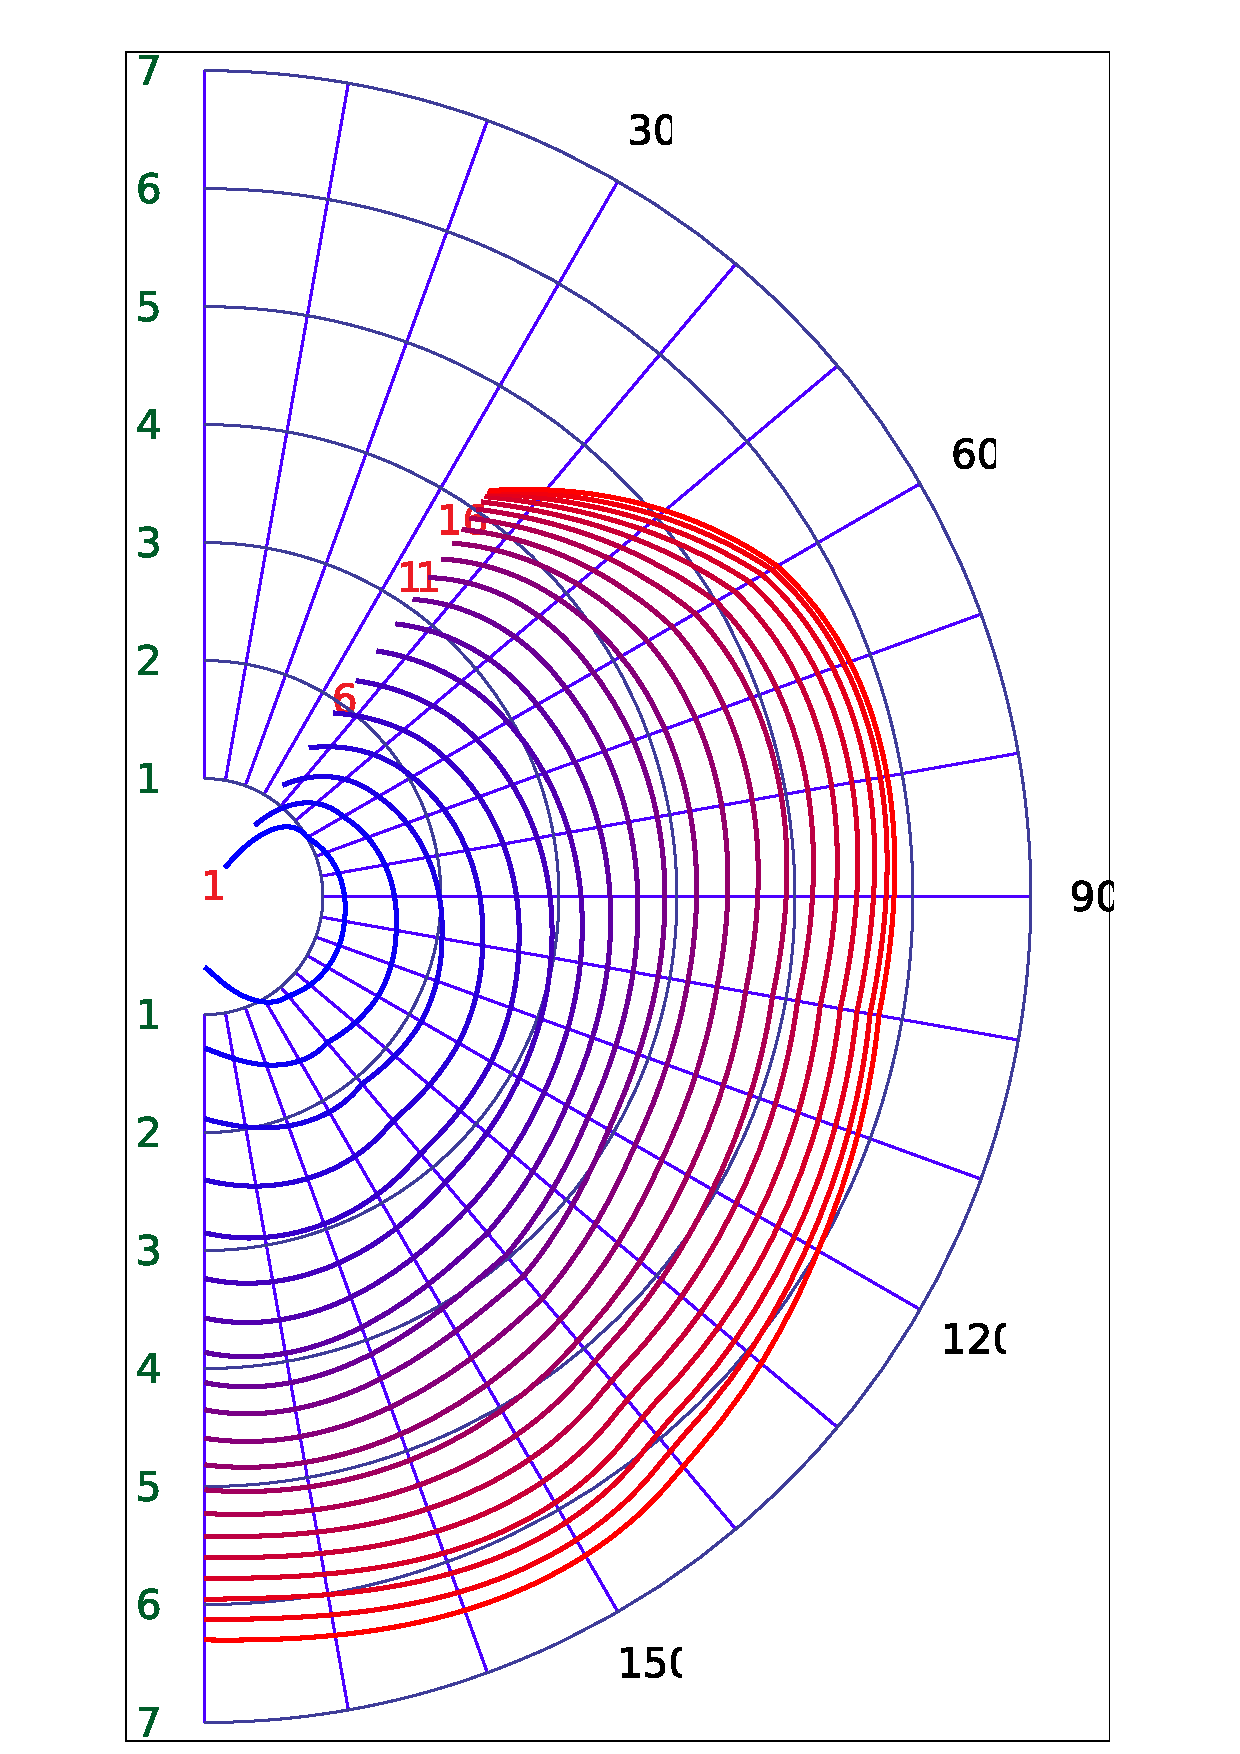
\includegraphics[width=6cm]{img/polardiagramm}
\caption{Polardiagramm eines Bootes, grün Windstärke in Knoten, rot
Geschwindigkeit in Knoten, schwarz Windangriffswinkel}
\label{polardiagram}
\end{wrapfigure}

Je nach Einfallswinkel des Windes variert die Schiffsgeschwindigkeit
stark. Bei frontal kommenden Wind fährt das Schiff gar nicht mehr
vorwärts und muss für diesen Umstand aufkreuzen, das heisst einen
Zickzack-Kurs fahren. Deshalb muss für jedes Schiff empirisch der
minimale Einfallswinkels vom Bug aus ermittelt werden, somit ist der
steilste Winkel bekannt.

Die Schiffsgeschwindigkeit variert aufgrund der physischen Eigenschaften
von Segel, Rumpf und Aerodynamik. Entgegen Intuition ist Wind von
Achtern nicht der schnellste, sondern bei sogenannt halben Wind (meist
zwischen 80\degree und 105\degree). Da sich diese Daten nicht nur bei
unterschiedlichen Einfallswinkel verändern, sondern auch bei
unterschiedlichen Windgeschwindigkeiten, empfiehlt es sich ein
sogenanntes Polardiagramm zu erstellen, dass die unterschiedliche
Fahrtgeschwindigkeiten in Bezug zu Einfallswinkel und
Windgeschwindigkeit darstellt.

Da aber der Datensatz nicht durchgehend ist, muss zwischen den bekannten
und ermittelten Punkten interpoliert werden.

\subsubsection{Interpolationsverfahren}
Um diese Daten zu interpolieren eignet sich die bilineare Interpolation
am besten, da sie sehr einfach zu implementieren ist, über eine für
unsere Zwecke genügend hohe Genauigkeit verfügt, in linearer Zeit
rechnet und nur aus Multiplikationen sowie Additionen besteht, was
aufgrund von den heutigen CPU-Befehlen nur noch wenigen Taktzyklen
braucht und somit zu einer sehr hohen Ausführgeschwindigkeit führt.

Andere Interpolationsmethoden wie qubische Interpolation,
Spline-Interpolation oder polynomielle Interpolation sind entweder zu
ressourcen konsumierend, langsam oder sogar instabil. Daher wurde diese
nicht in Betracht gezogen. Ausserdem verwendet dieses Verfahren nur die
unmittelbaren Nachbarwerte und kommt damit mit weniger Informationen
zurecht.

\subsection{Implementation}
\subsubsection{Eingabedaten-Parser}
Die Schiffsdaten sind als CSV\footnote{Comma Separated Values}-Datei
gegeben und werden von einem selbst\-geschriebenen Parser in ein
passendes Klassen-Konstrukt geladen. Die Schwierigkeit bestand darin,
dass die Daten nicht-dekoriert sind und daher nur durch ihre Position
von anderen Typen zu unterscheiden sind. Das bedeutet allerdings auch,
dass der Parser sich auf diese Datenstruktur verlässt und keine
Abweichungen duldet und sonst abstürzt.

Dieses Problem ist allerdings vertretbar, da die Datenstruktur
vorgegeben ist und der Parser daran angepasst wurde.

\subsubsection{Verarbeitungsklasse}
Die Klasse \texttt{BoatSpeedDiagram.java\footnote{Im Package 
ch.zhaw.lakerouting.interpolation.boatdiagram zu finden}} verwaltet das
Polardiagram und bietet die nötigen Methoden für die Abfrage der Werte
an, kapselt die Interpolation, so das der Programmierer sich darum nicht
kümmern muss.

\subsubsection{Bilineare Interpolation}
Die Interpolation an sich ist durch 
\begin{equation}
f(x,y) \approx \begin{bmatrix} 1-x & x \end{bmatrix} \begin{bmatrix}
f(0,0) & f(0,1) \\ f(1,0) & f(1,1) \end{bmatrix} \begin{bmatrix} 1 - y
\\ y \end{bmatrix}
\label{eq:bilineareinterpolation}
\end{equation}
geben und kann in Java wie nachfolgend gezeigt, implementiert werden.

 \lstinputlisting[label=src:bilinearinterpolation,caption=Bilineare Interpolation]{code/BilinearInterpolation.java}
Die konkrete Berechnung erfolgt auf den Zeilen 17-19 und zeigen den
einfachen Charakter der Berechnung. Diese Implementation erfordert
allerdings eine geringe Aufbereitung der Eingabewerte, ist dafür
einfacher zu testen und somit indirekt auch weniger anfällig für
Implementationsfehler, was direkt zu robusterem Code führt.

% Author: Mathias Hablützel

\section{Erfassung Windfelder}\label{s:windfields}

\subsection{Problemanalyse}
\subsubsection{Einlesen der Daten}
Die vorgegebenen Eingabedaten in einer einfachen, unstrukturierten
Text-Datei werden als Vektor eingelesen, zwei numerische Werte werden
jeweils als $u$- bzw. $v$-Komponente an einer bestimmten Position des
Vektors erfasst.

\subsubsection{Verwalten der Daten}
Da pro bestimmten Zeitpunkt ein bekanntes (prognostiziertes) Windfeld
bekannt ist, müssen mehrere Windfelder verwaltet werden können. Es kann
der Fall eintreten, an dem der Windvektor $a_{x,y,t}$ und der Windvektor
einer unmittelbar daneben liegenden Position an einem etwas späteren
Zeitpunkt gebraucht wird, also $a_{x+1,y,t+1}$ zum Beispiel. Somit
müssen die Positionsangaben vom Windfeld zu $t$ und $t+1$ identisch
sein. 

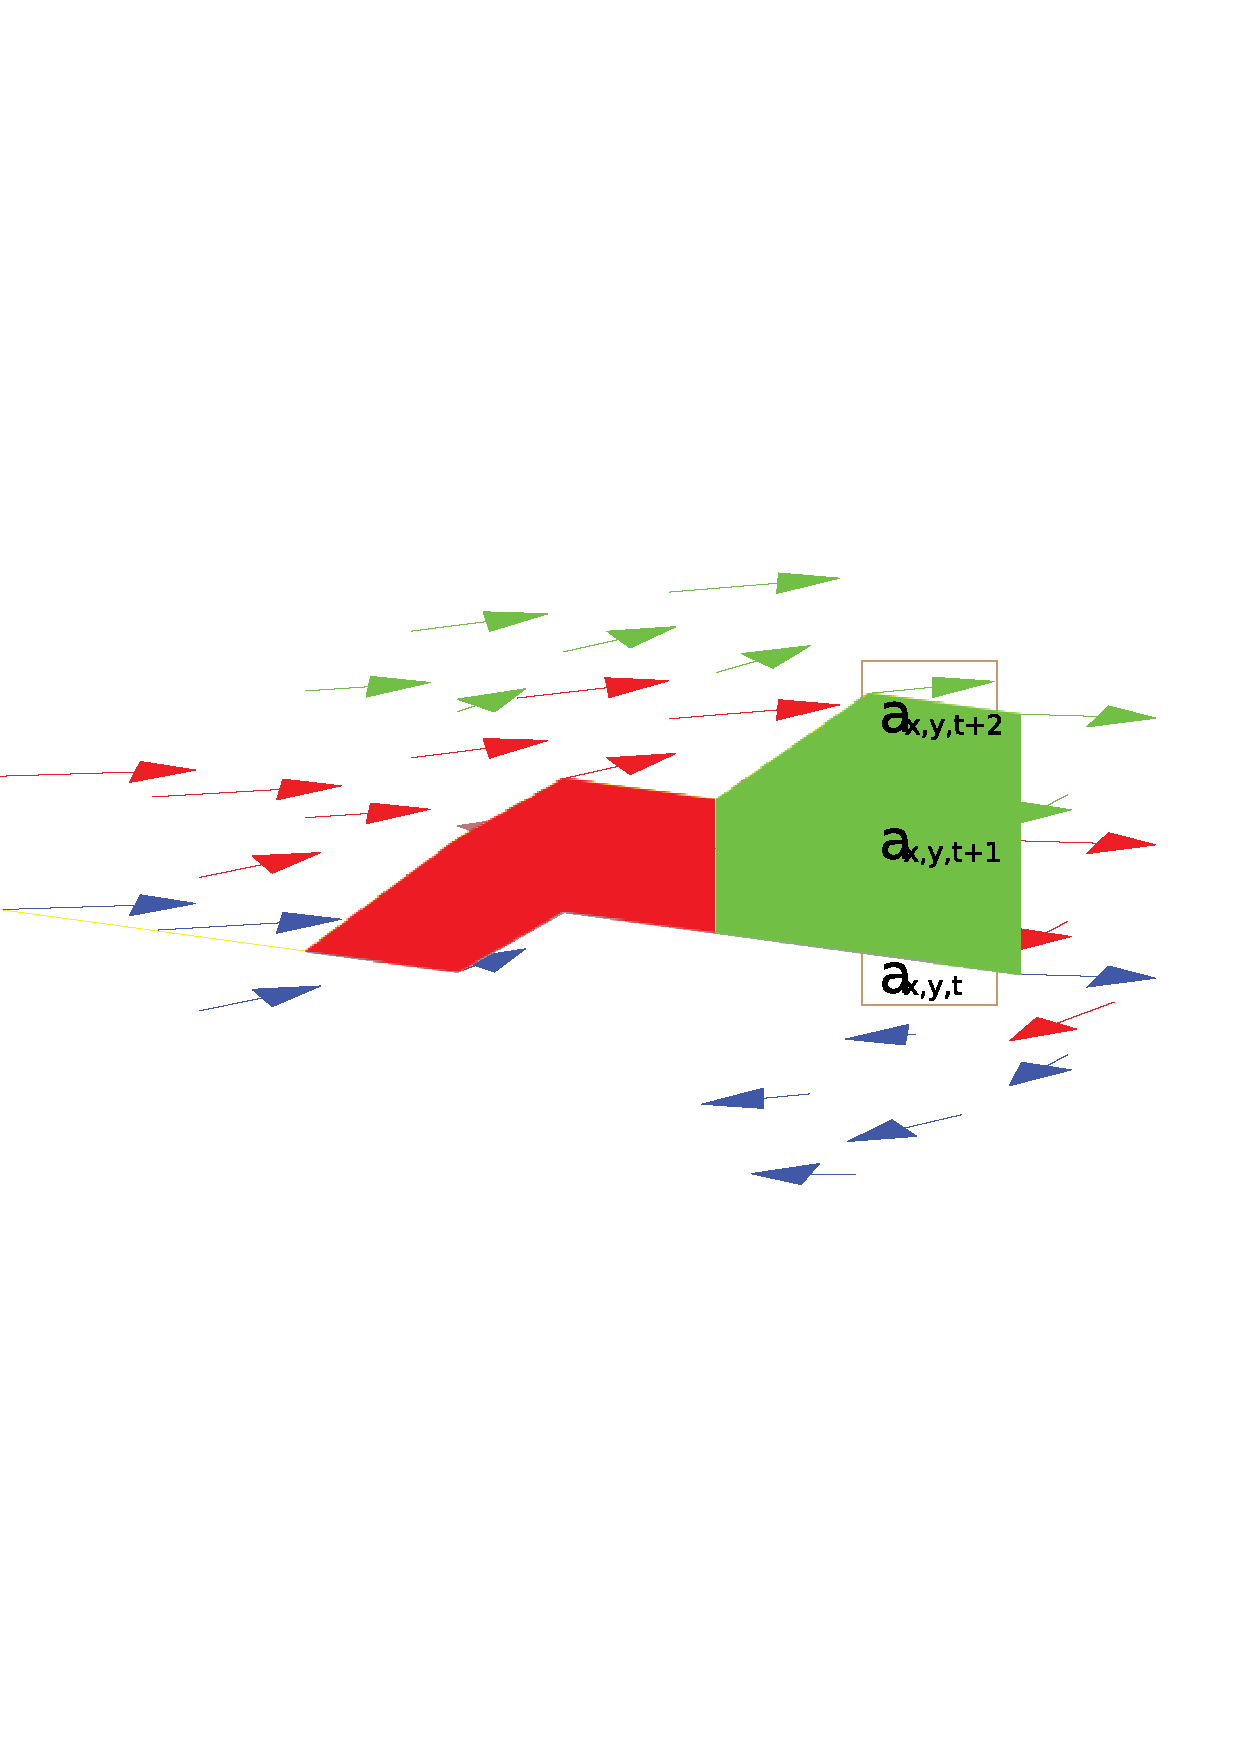
\includegraphics[width=12cm]{img/windfield-different-layer}

% Author: Mathias Hablützel

\section{Berechnung von Segelgeschwindigkeit anhand der Windfelder}
Die in Abschnitt \ref{s:windfields} eingelesenen Windfelder werden nun für die
Berechnung der Segelgeschwindigkeit verwendet. Gegen sind der
Windangriffswinkel auf das Schiff durch die Windvektoren von Punkt $A$ nach
$B$, die Segelrichtung ist damit auch bekannt.

% TODO: Skizze zeichnen mit Punkt A -> B, Segelboot, Windvektoren
 
\subsection{Geschwindigkeit am Ausgangspunkt}
Da es bekannt ist zu welcher Zeit man am Ausgangspunkt $A$ ist, weiss man auch
welcher Windvektor existiert (der sich ja mit der Zeit verändert). Somit lässt
sich die Geschwindigkeit des Bootes am Ausgangspunkt berechnen.

\subsection{Geschwindigkeit am Zielpunkt}
Hier besteht das Problem, dass es nicht bekannt ist, wann das Boot am Punkt $B$
ankommt, die Ankunftszeit hängt vom Windvektor $v_{1}$ in Punkt $A$ zur Zeit
$t_{1}$ und vom Windvektor $v_{2}$ in Punkt $B$ zur Zeit $t_{2}$ ab. $t_{2}$
ist unbekannt und folglich ist $v_{2}$ auch nicht bekannt (nur dessen Position
ist im Voraus bekannt).

Also muss in einem ersten Schritt die Ankunftszeit approximiert werden.  Wir
könnten die Euler'sche Regression verwenden, allerdings besteht hier das
Problem, dass der Algorithmus nicht zwingend die beste Lösung findet und über
eine unterschiedlich lange Laufzeit verfügt. Daher erschien ein zweischrittiges
Verfahren für eine Teilapproximation vernünftig, welches in linearer Zeit
ausgeführt werden kann.

\subsection{Berechnung der Ankunftszeit}
Vom Startpunkt $A$ ist die Uhrzeit, die Position und somit der Windvektor
bekannt. Daraus kann die Geschwindigkeit des Segelbootes bestimmt werden
(ausgehend von Punkt $A$). Diese Geschwindigkeit wird nun für die gesamte
Distanz angenommen und daraus resultiert eine ungefähre Ankunftszeit. Wir
nehmen hier an, dass das Windfeld zu einem späteren Zeitpunkt nicht so stark
ändert, dass unsere Berechnungen zu stark von einem vernünftigen Wert abweicht,
unter anderem weil dies der Natur von Windfeldern widersprechen würde.
Ausgenommen sind Extremsituationen wie Windhosen oder Tornados. Aber in solchen
Situationen wäre das Segeln auch nicht vernünftig.

\subsection{Kurs (Track)}
Die Geschwindigkeit des Segelschiffes hängt einerseits von der Intensität des Windes und andererseits von der Einfallswinkel des Windvektors ab. Damit der Einfallswinkel des Windvektors berechnet werden kann, muss bekannt sein, in welche Richtung das Segelschiff segelt. Die Berechnung des Kurses findet wie folgt statt: Zuerst wird ein Kreuzprodukt der zwei Vektoren vom Ursprung  \(\overrightarrow{A}\) und \(\overrightarrow{B}\) brerechnet. Das Resultat entspricht dann der Normalenvektor \(\overrightarrow{N}\), welche senkrecht zu der aufgespalteten Ebene von \(\overrightarrow{A}\) und \(\overrightarrow{B}\) steht. Danach wird wiederum ein Kreuzprodukt berechnet, diesmal aber vom Vektor \(\overrightarrow{A}\) und dem Normalenvektor \(\overrightarrow{N}\). Dies ergibt als Resultat die Richtung des Segelschiffes. Da dieser Vektor aber 3-dimensional ist, muss sie auf die lokale Tangentialebene (\(\overrightarrow{e_{\theta}}\), \(\overrightarrow{e_{\phi}}\)) des Punktes $A$ projiziert werden, damit wir ein 2-dimensionales Vektor kriegen. \\
Die grafische Darstellung dieser Berechnung sieht wie folgt aus:
\begin{figure}[h!]
\centering
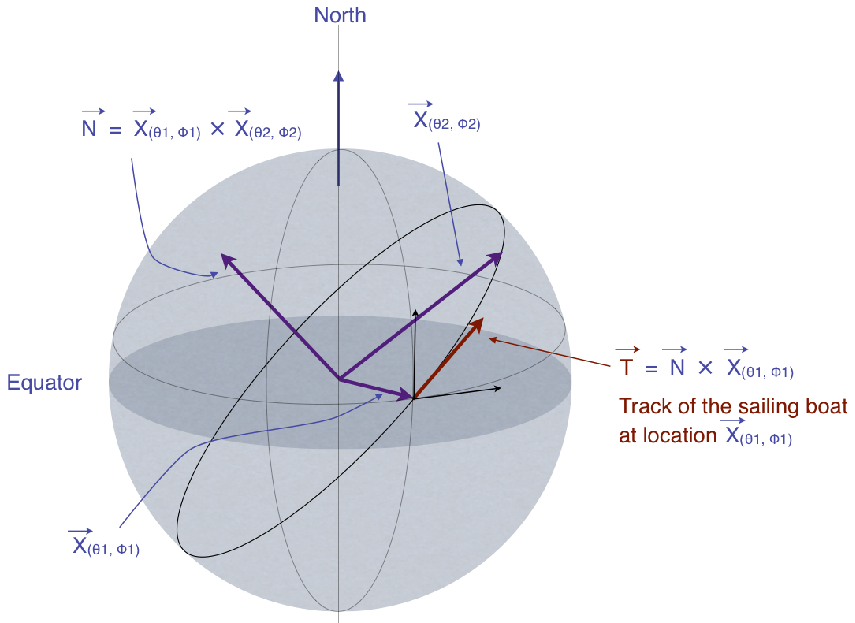
\includegraphics[width=0.8\linewidth]{img/track}
\caption{Berechnung des Kurses}
\label{gridnetConn}
\end{figure}

\subsection{Implementation}
In der Implementation haben wir einen noch einfacheren Ansatz verfolgt:

%\begin{align}
%t = \frac{1}{2} (\frac{2d}{|\mathbf{\overrightarrow{v_{1}}} + \mathbf{\overrightarrow{v_{2}}}|})
%\end{align}

% Siehe letzte SEITE vom PDF "Navigation_Commented_New.pdf"!!!!!
\begin{align}
t = \frac{2d}{\mathbf{s_{1}} + \mathbf{s_{2}}}
\end{align}

t Reisezeit, d Distanz zwischen zwei Punkten, 
$s_{1}$ bzw. $s_{2}$ Schiffsgeschwindigkeit einmal mit Windvektor $v_{1}$ und einmal mit $v_{2}$.

\vspace{0.5cm}
% Im Kapitel 9.1.1 wird es erwähnt... Hier noch ref einfügen!
Würde der Windvektor $v_{2}$ aufgrund von der absoluten Zeit, also in
Bezug zur Uhrzeit, auf das Windfeld des nächsten Zeitabschnitts fallen,
so wird $v_{2}$ mit dem des (zeitlich) nächsten Windfeldes ersetzt.

\newpage
\part{Resultate}

\section{GraphList}
Wie in Abschnitt \ref{aufg6:entscheidungsbaum} erklärt wurde, brauchen wir eine Liste, die alle nötigen Informationen zu den Knoten beinhaltet. Da die Grösse des Arrays variabel ist und wir zum grössten Teil einen index-basierten Zugriff benötigen, haben wir uns entschieden die Datnestruktur $java.util.ArrayList$ mit Generics zu verwenden. Eine generische ArrayList erlaubt es genau zu definieren, welche Elemente/Datentypen einer ArrayList hinzugefügt werden dürfen. Ausserdem brauchen wir für eine tabellarische Form ein 2-dimensionales ArrayList. Um dies zu erreichen, wird ein ArrayList in einem ArrayList definiert. Somit entspricht der erste ArrayList der Spalten und die zweite der Zeilen dieser Spalten. \\
Dementsprechend sieht die Initialisierung des ArrayLists so aus:

\lstinputlisting[label=src:graphListInitialization,caption=Initialisierung der Liste]{code/graphlist_initialize.java}

\subsection{Node}
Für die Speicherung der Daten wurde eine Klasse $Node$ erstellt, welche die Werte über die Knoten beinhaltet. Weil wir nun mehrere Informationen zu den einzelnen Knoten haben, haben wir uns entschieden, neben den Auflistungen in \ref{aufg6:entscheidungsbaum} auch noch weitere Daten in der Liste abzuspeichern, um Redundanz zu vermeiden. Deshalb werden neu auch Koordinaten zu den Knoten und die dazugehörigen Windvektoren in der Liste abgelegt. \\
Demzufolge enthält die Klasse folgende Informationen:
\begin{itemize}
\item \textbf{TimeOfArrival}: Die Dauer vom Anfangsknoten bis zu diesem Knoten.
\item \textbf{Previous Node}: Die Referenz zum vorherigen Knoten.
\item \textbf{Coordinate}: Breiten- und Längengrade des Knotens.
\item \textbf{WindVektor}: Der Windvektor $(u, v)$ an diesem Knoten.
\end{itemize}

Desweiteren erbt diese Klasse von der Interface $Comparable$, um Vergleiche zwischen den Knoten zu ermöglichen. Infolgedessen ist es möglich, die Klasse $Collections$ zu benutzen, welche nützliche Methoden für Listen wie $min()$, $max()$, $sort()$ etc. enthält. Wir machen in unserem Code von der $min()$-Methode Gebrauch, um den Knoten mit dem kleinsten TimeOfArrival in einer Spalte zu finden. \\

Als nächstes wurde innerhalb der ArrayList eine sogenannte LinkedList implementiert. Jeder Knoten beinhaltet eine Referenz zum vorherigen Knoten und der Anfangsknoten hat eine Referenz auf sich selbst. Dementsprechend braucht man nicht durch alle Knoten zu iterieren um einen Pfad zu zeichnen, sondern es reicht den Knoten zu wählen, von dem man den Pfad zum Anfang zeichnen möchte. \\

Die Implementation der Klasse Node sieht wie folgt aus:

\lstinputlisting[label=src:nodeClass,caption=Node-Class]{code/node.java}

\section{Polar-Diagramm}
\subsection{Parser}
Die Schiffsdaten sind als CSV\footnote{Comma Separated Values}-Datei gegeben
und werden von einem selbst\-geschriebenen Parser in ein passendes
Klassen-Konstrukt geladen. Die Schwierigkeit bestand darin, dass die Daten
nicht-dekoriert sind und daher nur durch ihre Position von anderen Typen zu
unterscheiden sind. Das bedeutet allerdings auch, dass der Parser sich auf
diese Datenstruktur verlässt und keine Abweichungen duldet und sonst abstürzt.

Dieses Problem ist allerdings vertretbar, da die Datenstruktur vorgegeben ist
und der Parser daran angepasst wurde. Es ist im Allgemeinen sehr schwierig
einen Parser für eine schwach typisierte Datenstruktur zu schreiben. Eine
robustere Datenstruktur würde XML bieten, die strikte Einschränkung bis hin zu
Datentypen für einzelne Felder bietet.

\subsection{Verarbeitungsklasse}
Die Klasse \texttt{BoatSpeedDiagram.java\footnote{Im Package
ch.zhaw.lakerouting.interpolation.boatdiagram zu finden}} verwaltet das
Polardiagram und bietet die nötigen Methoden für die Abfrage der Werte an,
kapselt die Interpolation, so das der Programmierer sich darum nicht kümmern
muss.

\subsection{Bilineare Interpolation}\label{sss:bilinearinterpolation}
Die Interpolation an sich ist durch 
\begin{equation}
f(x,y) \approx \begin{bmatrix} 1-x & x \end{bmatrix} \begin{bmatrix}
f(0,0) & f(0,1) \\ f(1,0) & f(1,1) \end{bmatrix} \begin{bmatrix} 1 - y
\\ y \end{bmatrix}
\label{eq:bilineareinterpolation}
\end{equation}
geben und kann in Java wie nachfolgend gezeigt, implementiert werden.

 \lstinputlisting[label=src:bilinearinterpolation,caption=Bilineare Interpolation]{code/BilinearInterpolation.java}
Die konkrete Berechnung erfolgt auf den Zeilen 17-19 und zeigen den einfachen
Charakter der Berechnung. Diese Implementation erfordert allerdings eine
geringe Aufbereitung der Eingabewerte, ist dafür einfacher zu testen und somit
indirekt auch weniger anfällig für Implementationsfehler, was direkt zu
robusterem Code führt.

\section{Windfelder}
Die Implementation ist vergleichsweise einfach gehalten und besteht aus einer
Klasse für ein einzelnes Windfeld mit Hilfsfunktionalitäten für die
Interpolation der Windvektoren und das Abfragen der Nachbarsvektoren an einer
bestimmten Position. Diese einzelnen Windfelder werden dann in einem Art Stapel
aufbewahrt\footnote{Wir verwenden der Einfachheit halber ein normales Array.}
Im Prinzip besteht das alles aus einer dreidimensionalen Struktur aus
Windvektoren.

\subsection{Windfeld-Parser}
Der Parser ist ein Eigenbau und wurde speziell für diese Datenstruktur
geschaffen. Diverse Unzulänglichkeiten wie nicht-leere Zeilen und Trailing
Spaces haben die Entwicklung erschwert und dementsprechend viel Zeit gekostet.

Allerdings lässt sich der Parser leicht auf andere Ressourcen erweitern wie zum
Beispiel HTTP und erlaubt auch die direkte Anbindung an Datenbanken.

\subsection{Interpolation der Windvektoren}
Da das Windfeld und das Entscheidungsnetz nicht über dieselben Koordinaten
verfügen und dementsprechend die Entscheidungspunkte normalerweise zwischen den
Windvektoren zu liegen kommen, wird nach Berechnung des Entscheidungsnetzes dem
Windfeld die Koordinatenliste übergeben. Das Windfeld interpoliert die
Windrichtung bzw. die Windvektoren an den geforderten Positionen. Das erfolgt
wie bereits in Abschnitt \ref{sss:bilinearinterpolation} erklärt über dieselbe
Klasse.

Nach dieser initialen Interpolation verfügen das Entscheidungsnetz und das
Windfeld über dieselben Array-Indizes und können somit leicht (wieder-)
verwendet werden.


\subsection{Klassendiagramm}
% Klassen mit Beziehungen zueinander aufzeigen.

\subsection{Logging}
% Kurz Logging erklären. (ggf. PA anschauen :))

\subsection{JavaDoc}
% Wie JavaDoc zu bedienen sei und was alles dort drin steht.

\section{Testing}
\subsection{Beispiele}
% Mit sinnvollen Beispielen simulieren.

\newpage
\part{Diskussion und Ausblick}
% Interpretation und Validierung der Resultate

\section{Erweiterbarkeit}
% Zeigen, dass es leicht erweiterbar und wiederverwendbar ist.
\subsection{Parallelisierung}
% Aufzeigen, dass Paralellisierung möglich ist.
\subsection{Weitere Datenquellen}
% Wie weitere Datenquellen eingesetzt werden können (z.B. HTTP anstatt Datei)
\subsection{Website}
% Wie daraus eine Webseite gemacht werden kann. Apps?

\section{Programmiertechnische Grenzen}
% (Im Sitzungsprotokoll vom 06.03.2012, Punkt 3)
% Im Bericht sollte ein Absatz vorhanden sein, welches die 
% programmiertechnischen Grenzen oder Genauigkeiten der mathematischen 
% Funktionen wie Sinus/Cosinus, Datentypen etc. behandelt und diskutiert. 

\section{Optimierungsmöglichkeiten}
\subsection{Sonderfälle}
% Das Problem mit Spread ausdiskutieren
% Grössere Distanzen

\section{Erkenntnisse}
\subsection{Schlussfolgerung}
\subsection{Arbeitsrevue}

\newpage
\part{Anhang}

\section{Projektplanung}

\subsection{Projektübersicht}

\subsubsection{Benötigte Ressourcen}
\begin{itemize}
\item Menschliche Ressourcen \\
Das Projekt wird von 2 Personen für rund 1 Semester mit der Betreuung
eines Dozenten gemäss dem Auftrag des Auftraggebers durchgeführt. Auch
seitens des Auftraggebers steht ein Betreuer zu Verfügung, den wir bei
Unklarheiten ebenfalls kontaktieren können und von dem wir auch die
nötigen Unterlagen zugeschickt bekommen. Ausserdem steht auch ein
Nebenbetreuer zur Verfügung, der grundsätzlich für IT spezifische Fragen
zuständig ist. Es wird davon ausgegangen, dass alle Projektmitglieder
durchschnittlich 20 bis 25 Stunden pro Woche am Projekt arbeiten.

\item Räume \\
Es werden keine speziellen Räume gebraucht. Aber für eine bessere,
verstärkte und erfolgreiche Zusammenarbeit wurde das Zimmer TE616 in der
ZHAW-Schulgebäude reserviert. Ausserdem werden einmal die Woche, jeweils
am Dienstag, zwei Zimmer der Abteilung Wetterdienst in der
MeteoSchweiz-Gebäude benutzt. Jedoch wird das Projekt weitgehend als
virtuelle Organisation geführt, das heisst, dass der physische Standort
der Teilnehmer nicht von Bedeutung ist.

\end{itemize}

\subsubsection{Meetings}
Die Kommunikation im Projekt mit den beiden Betreuer erfolgt in Form von ordentlichen Meetings jeden Dienstag in der Hauptgebäude der MeteoSchweiz in Zürich. Bei Bedarf kann sie auch per E-Mail oder ausserordentlichen Sitzungen stattfinden. Ausserdem wurde für das Projekt 4 Meilensteine definiert, welche dann anstelle der wöchentlichen Sitzungen stattfinden werden. Die Meilensteine liegen bewusst vor dem eigentlichen Abgabetermin, um Pufferzeiten zu schaffen.

\subsubsection{Kontaktdaten des Auftraggebers}
MeteoSchweiz\\
Eidgenössisches Departement des Innern EDI \\
Bundesamt für Meteorologie und Klimatologie\\
Krähbühlstrasse 58\\
CH-8044 Zürich\\
Tel.   +41 44 256 91 11 \\
Fax   +41 44 256 92 78\\

\subsection{Vorgehensmodell}
%Unvollständig
Für unser Projekt haben wir uns für das V-Modell entschieden, da die
Phasen stabile Anforderungen haben und sie wenig Management-Aufwand
benötigen. Desweiteren besitzen sie klare Abgrenzungen und der Umfang
der Arbeit ist klar abschätzbar. 

\subsection{Zeitliche Planung}
%Unvollständig
\subsubsection{Effektiver Ablauf}
\begin{table}[h!]
\centering 
  \begin{tabular}{| c | l | r | >{\color{red}} r |}
    \hline
    \rowcolor{hellgrau} 
    \textbf{Arbeitspakete} & \textbf{Tasks} & \textbf{Zeitaufwand} & \textbf{\color{black}Effektiv} \\ \hline \hline
    \multirow{1}{*}{} & \textbf{Planung} & \textbf{Tage} & \textbf{Tage}  \\ \cline{2-4} \hline \hline
     & \textbf{Implementierung} & \textbf{Tage} & \textbf{Tage}  \\ \hline
     \multirow{1}{*}{Nr. 1}& Aufgabe 1+2 & 12 Tage & 12 Tage \\ \hline
     Nr. 2 & Aufgabe 3 & 8 Tage & 8 Tage \\ \hline
     Nr. 3& Aufgabe 4 & 8 Tage & 25 Tage \\ \hline
     Nr. 4& Aufgabe 5 & 13 Tage & 10 Tage \\ \hline
     Nr. 5& Aufgabe 6 & 15 Tage &  Tage \\ \hline
     Nr. 6& Aufgabe 7 & 22 Tage &  Tage \\ \cline{2-4}\hline \hline
     Nr. 7& \textbf{Testing / Finetuning} & \textbf{ Tage} & \textbf{ Tage}  \\ \hline \hline
     \multirow{3}{*}{Nr. 8} & \textbf{Erkenntnis} & \textbf{ Tage} & \textbf{ Tage} \\ \cline{2-4}
     & Schlussfolgerung &  Tage &  Tage  \\ \cline{2-4}
     & Arbeitsrevue &  Tage &   Tage \\ \cline{2-4} \hline \hline
     & \textbf{Reserve} & \textbf{10 Tage} & \textbf{ Tage} \\ \hline \hline \hline
     & \textbf{Zeitaufwand insgesamt} & \textbf{ Tage}  & \textbf{ Tage} \\ \hline \hline
  \end{tabular}
  \caption{Projektplan Ablauf}
  \label{EffektivPlan}
\end{table}

\paragraph{Definition}
1 Tag = 5 Arbeitsstunden pro Person \\

\subsubsection{Gantt-Diagramm}
\begin{figure}[h!]
\centering
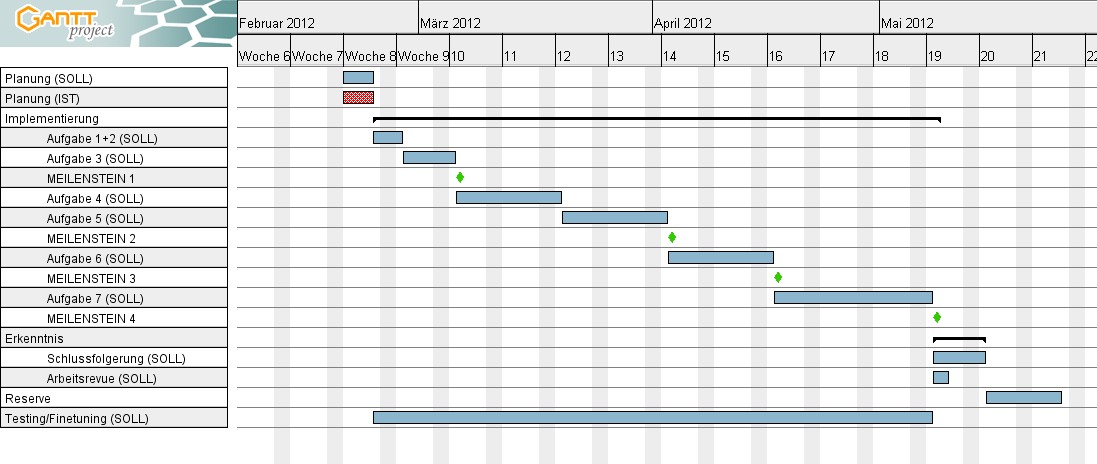
\includegraphics[width=0.8\linewidth]{img/projektplanung.png}
\caption{Projektplan}
\label{prplan}
\end{figure}

\subsubsection{Arbeitspakete}
Im Folgenden wird das Projekt in Arbeitspakete und ihre Abhängigkeiten eingeteilt, wie es auch in der Tabelle \ref{EffektivPlan} ersichtlich ist. Die Pakete wurden so gewählt, dass sie genau eine geschlossene Aufgabenstellung beschreiben und die Abhängigkeiten definieren, welche Arbeitspakete abgeschlossen sein müssen, damit ein bestimmtes Arbeitspaket begonnen werden kann. Desweiteren wurden auch die geplanten Dauer der Arbeitspakete angegeben. \\

Es ist festgelegt, dass beide Projektmitglieder auch gleichzeitig die
Projektleiter für die gesamte Projektlaufzeit sind. Es wird aber im
Verlauf des Projektes in jeder einzelnen Phase jeweils ein
Projektmitglied die eigentliche Projektleitung übernehmen.

Der Projektleiter der jeweiligen Phase ist hauptverantwortlich für die
rechtzeitige Fertigstellung und die Qualität des Produkts der jeweiligen
Phase.

\begin{table}[h!]
\centering 
  \begin{tabularx}{\textwidth}{| l | X | l| X | }
    \hline
    \cellcolor{hellgrau}\textbf{Nummer} & \multicolumn{3}{l |}{1}  \\ \hline
    \cellcolor{hellgrau}\textbf{Bezeichnung} & \multicolumn{3}{l |}{Aufgabe 1 \& 2} \\ \hline       
    \cellcolor{hellgrau} & \multicolumn{3}{l |}{•	Erstellung eines Entscheidungsnetzes auf der Erdkugel}  \\ 
    \cellcolor{hellgrau} & \multicolumn{3}{l |}{•	Berechnung einer Orthodromie} \\ 
    \cellcolor{hellgrau} & \multicolumn{3}{l |}{(Distanz in Meilen zwischen zwei Punkten auf der Erdkugel)}  \\ 
    \cellcolor{hellgrau} & \multicolumn{3}{l |}{•	Erstellung der Koordinatendatei eines Sees (in Koordinaten)}  \\ \cline{2-4}
    \cellcolor{hellgrau} & \multicolumn{3}{l |}{•	Erstellung eines Entscheidungskernes in dynamische Programmierung}  \\ 
     \multirow{-6}{*}{\textbf{\cellcolor{hellgrau}Beschreibung}} & \multicolumn{3}{l |}{•	Berechnung von Orthodromien auf der Erdoberfläche mit Testdaten} \\ \hline
    \cellcolor{hellgrau}\textbf{Start} & 24.02.2012 &  \cellcolor{hellgrau}\textbf{Ende} & 06.03.2012\\ \hline
    \cellcolor{hellgrau}\textbf{Abhängigkeiten} & Keine&  \cellcolor{hellgrau}\textbf{Verantwortung} & Fevzi Yükseldi\\ \hline
  \end{tabularx}
  \caption{Arbeitspaket 1}
\end{table}

\begin{table}[h!]
\centering 
  \begin{tabularx}{\textwidth}{| l | X | l| X | }
    \hline
    \cellcolor{hellgrau}\textbf{Nummer} & \multicolumn{3}{l |}{2}  \\ \hline
    \cellcolor{hellgrau}\textbf{Bezeichnung} & \multicolumn{3}{l |}{Aufgabe 3} \\ \hline       
    \cellcolor{hellgrau} & \multicolumn{3}{l |}{•	Erfassung des Polardiagramms eines Segelschiffes}  \\ 
    \cellcolor{hellgrau} & \multicolumn{3}{l |}{•	Interpolationsverfahren} \\ 
     \multirow{-3}{*}{\textbf{\cellcolor{hellgrau}Beschreibung}} & \multicolumn{3}{l |}{•	Test: Schiffgeschwindigkeiten berechnen} \\ \hline
    \cellcolor{hellgrau}\textbf{Start} & 06.03.2012 &  \cellcolor{hellgrau}\textbf{Ende} & 13.03.2012\\ \hline
    \cellcolor{hellgrau}\textbf{Abhängigkeiten} & Keine&  \cellcolor{hellgrau}\textbf{Verantwortung} & Mathias Hablützel\\ \hline
  \end{tabularx}
  \caption{Arbeitspaket 2}
\end{table}

\begin{table}[h!]
\centering 
  \begin{tabularx}{\textwidth}{| l | X | l| X | }
    \hline
    \cellcolor{hellgrau}\textbf{Nummer} & \multicolumn{3}{l |}{3}  \\ \hline
    \cellcolor{hellgrau}\textbf{Bezeichnung} & \multicolumn{3}{l |}{Aufgabe 4} \\ \hline       
    \cellcolor{hellgrau} & \multicolumn{3}{l |}{•	Erfassung des Windfeldes. Quelle: stündliche Vorhersagedaten des COSMO-2 Modells}  \\ 
    \cellcolor{hellgrau} & \multicolumn{3}{l |}{•	Interpolation auf das Entscheidungsnetzes (zwei mögliche Methoden)} \\ 
     \multirow{-3}{*}{\textbf{\cellcolor{hellgrau}Beschreibung}} & \multicolumn{3}{l |}{•	Test: Darstellung des Windfeldes auf dem Entscheidungsnetz für eine Vorhersagefrist.} \\ \hline
    \cellcolor{hellgrau}\textbf{Start} & 13.03.2012 &  \cellcolor{hellgrau}\textbf{Ende} & 20.03.2012\\ \hline
    \cellcolor{hellgrau}\textbf{Abhängigkeiten} & Keine&  \cellcolor{hellgrau}\textbf{Verantwortung} & Mathias Hablützel \\ \hline
  \end{tabularx}
  \caption{Arbeitspaket 3}
\end{table}

\begin{table}[h!]
\centering 
  \begin{tabularx}{\textwidth}{| l | X | l| X | }
    \hline
    \cellcolor{hellgrau}\textbf{Nummer} & \multicolumn{3}{l |}{4}  \\ \hline
    \cellcolor{hellgrau}\textbf{Bezeichnung} & \multicolumn{3}{l |}{Aufgabe 5} \\ \hline       
    \cellcolor{hellgrau} & \multicolumn{3}{l |}{•	Wechselwirkung Windfeld – Segelschiff}  \\ 
    \cellcolor{hellgrau} & \multicolumn{3}{l |}{•	Geometrie um das Schiff, Ableitung dessen Geschwindigkeit} \\ 
     \multirow{-3}{*}{\textbf{\cellcolor{hellgrau}Beschreibung}} & \multicolumn{3}{l |}{•	Test: Berechnung der Schiffgeschwindigkeit im Windfeld} \\ \hline
    \cellcolor{hellgrau}\textbf{Start} & 20.03.2012 &  \cellcolor{hellgrau}\textbf{Ende} & 03.04.2012\\ \hline
    \cellcolor{hellgrau}\textbf{Abhängigkeiten} & Arbeitspakete 2 \& 3 &  \cellcolor{hellgrau}\textbf{Verantwortung} & Fevzi Yükseldi\\ \hline
  \end{tabularx}
  \caption{Arbeitspaket 4}
\end{table}

\begin{table}[h!]
\centering 
  \begin{tabularx}{\textwidth}{| l | X | l| X | }
    \hline
    \cellcolor{hellgrau}\textbf{Nummer} & \multicolumn{3}{l |}{5}  \\ \hline
    \cellcolor{hellgrau}\textbf{Bezeichnung} & \multicolumn{3}{l |}{Aufgabe 6} \\ \hline       
    \cellcolor{hellgrau} & \multicolumn{3}{l |}{•	Erweiterung des geometrischen Entscheidungskerns}  \\ 
    \cellcolor{hellgrau} & \multicolumn{3}{l |}{~~~~~o	Zeitmanagement} \\ 
    \cellcolor{hellgrau} & \multicolumn{3}{l |}{~~~~~o	Rekursion} \\ 
     \multirow{-4}{*}{\textbf{\cellcolor{hellgrau}Beschreibung}} & \multicolumn{3}{l |}{•	Erstellung eines Entscheidungsbaums und Test} \\ \hline
    \cellcolor{hellgrau}\textbf{Start} & 03.04.2012 &  \cellcolor{hellgrau}\textbf{Ende} & 17.04.2012\\ \hline
    \cellcolor{hellgrau}\textbf{Abhängigkeiten} & Arbeitspakete 1 \& 4 &  \cellcolor{hellgrau}\textbf{Verantwortung} & Fevzi Yükseldi\\ \hline
  \end{tabularx}
  \caption{Arbeitspaket 5}
\end{table}

\begin{table}[h!]
\centering 
  \begin{tabularx}{\textwidth}{| l | X | l| X | }
    \hline
    \cellcolor{hellgrau}\textbf{Nummer} & \multicolumn{3}{l |}{6}  \\ \hline
    \cellcolor{hellgrau}\textbf{Bezeichnung} & \multicolumn{3}{l |}{Aufgabe 7} \\ \hline       
    \cellcolor{hellgrau} & \multicolumn{3}{l |}{•	Im Entscheidungsbaum Rückberechnung der optimalen Route}  \\ 
    \cellcolor{hellgrau} & \multicolumn{3}{l |}{•	Erstellung eines Logbuchs} \\ 
     \multirow{-3}{*}{\textbf{\cellcolor{hellgrau}Beschreibung}} & \multicolumn{3}{l |}{•	Graphische Darstellung  See, Windfeld, Entscheidungsbaum, optimale Route} \\ \hline
    \cellcolor{hellgrau}\textbf{Start} & 17.04.2012 &  \cellcolor{hellgrau}\textbf{Ende} & 08.05.2012\\ \hline
    \cellcolor{hellgrau}\textbf{Abhängigkeiten} & Arbeitspakete 1 \& 3 \& 5 &  \cellcolor{hellgrau}\textbf{Verantwortung} & \\ \hline
  \end{tabularx}
  \caption{Arbeitspaket 6}
\end{table}

\begin{table}[h!]
\centering 
  \begin{tabularx}{\textwidth}{| l | X | l| X | }
    \hline
    \cellcolor{hellgrau}\textbf{Nummer} & \multicolumn{3}{l |}{7}  \\ \hline
    \cellcolor{hellgrau}\textbf{Bezeichnung} & \multicolumn{3}{l |}{Testing / Finetuning} \\ \hline       
    \cellcolor{hellgrau} & \multicolumn{3}{l |}{•	Die Tests werden laufend durchgeführt.}  \\ 
     \multirow{-2}{*}{\textbf{\cellcolor{hellgrau}Beschreibung}} & \multicolumn{3}{l |}{•	Am Ende jedes Pakets wird die Arbeit mit realen Daten getestet} \\ \hline
    \cellcolor{hellgrau}\textbf{Start} & 24.02.2012 &  \cellcolor{hellgrau}\textbf{Ende} & 08.05.2012\\ \hline
    \cellcolor{hellgrau}\textbf{Abhängigkeiten} & Keine &  \cellcolor{hellgrau}\textbf{Verantwortung} & Alle \\ \hline
  \end{tabularx}
  \caption{Arbeitspaket 7}
\end{table}

\section{Offizielle Aufgabenstellung}

\section{Besprechungsprotokolle}


\bibliographystyle{ba_zhaw}
\bibliography{hablumat_biblio,yuksefev_biblio}
 \end{document}
